\begin{center}
                                \tablehead{\hspace{1cm}\\}
                                \tabletail{\hspace{1cm}\\}
                                \begin{supertabular}{p{0.5\textwidth}p{0.5\textwidth}}
                                \shrinkheight{1in}
                                \multicolumn{2}{p{\textwidth}}{The following bar charts show how frequently various types of maintenance issue -- including compactor-related problems, pest problems, and plumbing issues -- occur in compactor locations consolidation-wide as well as at major developments.} \\
                                \multicolumn{2}{c}{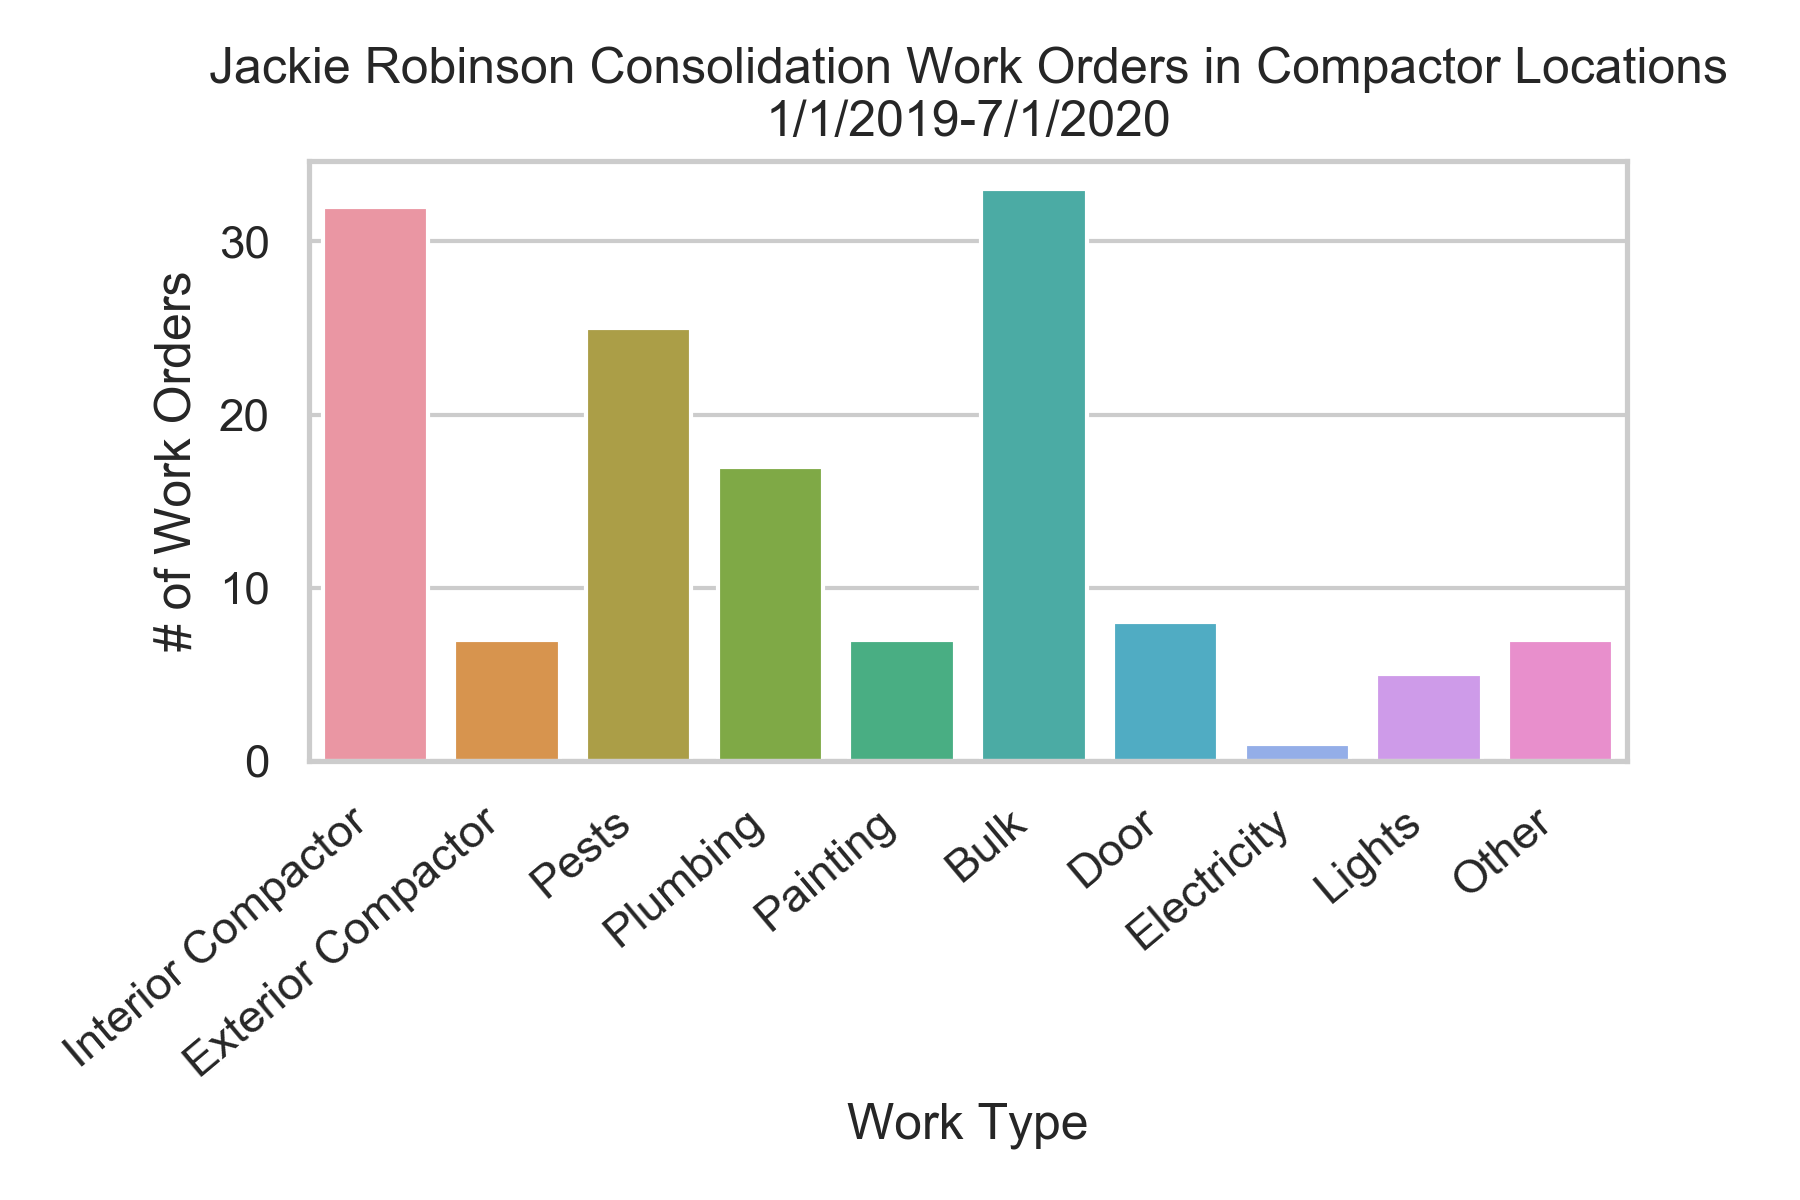
\includegraphics[width=0.6\textwidth]{\rootpath/WORK_ORDER_ANALYSIS/Consolidation_BarCharts/png/241_Jackie-Robinson_WorkOrder_Category_BarChart.png}} \\
                                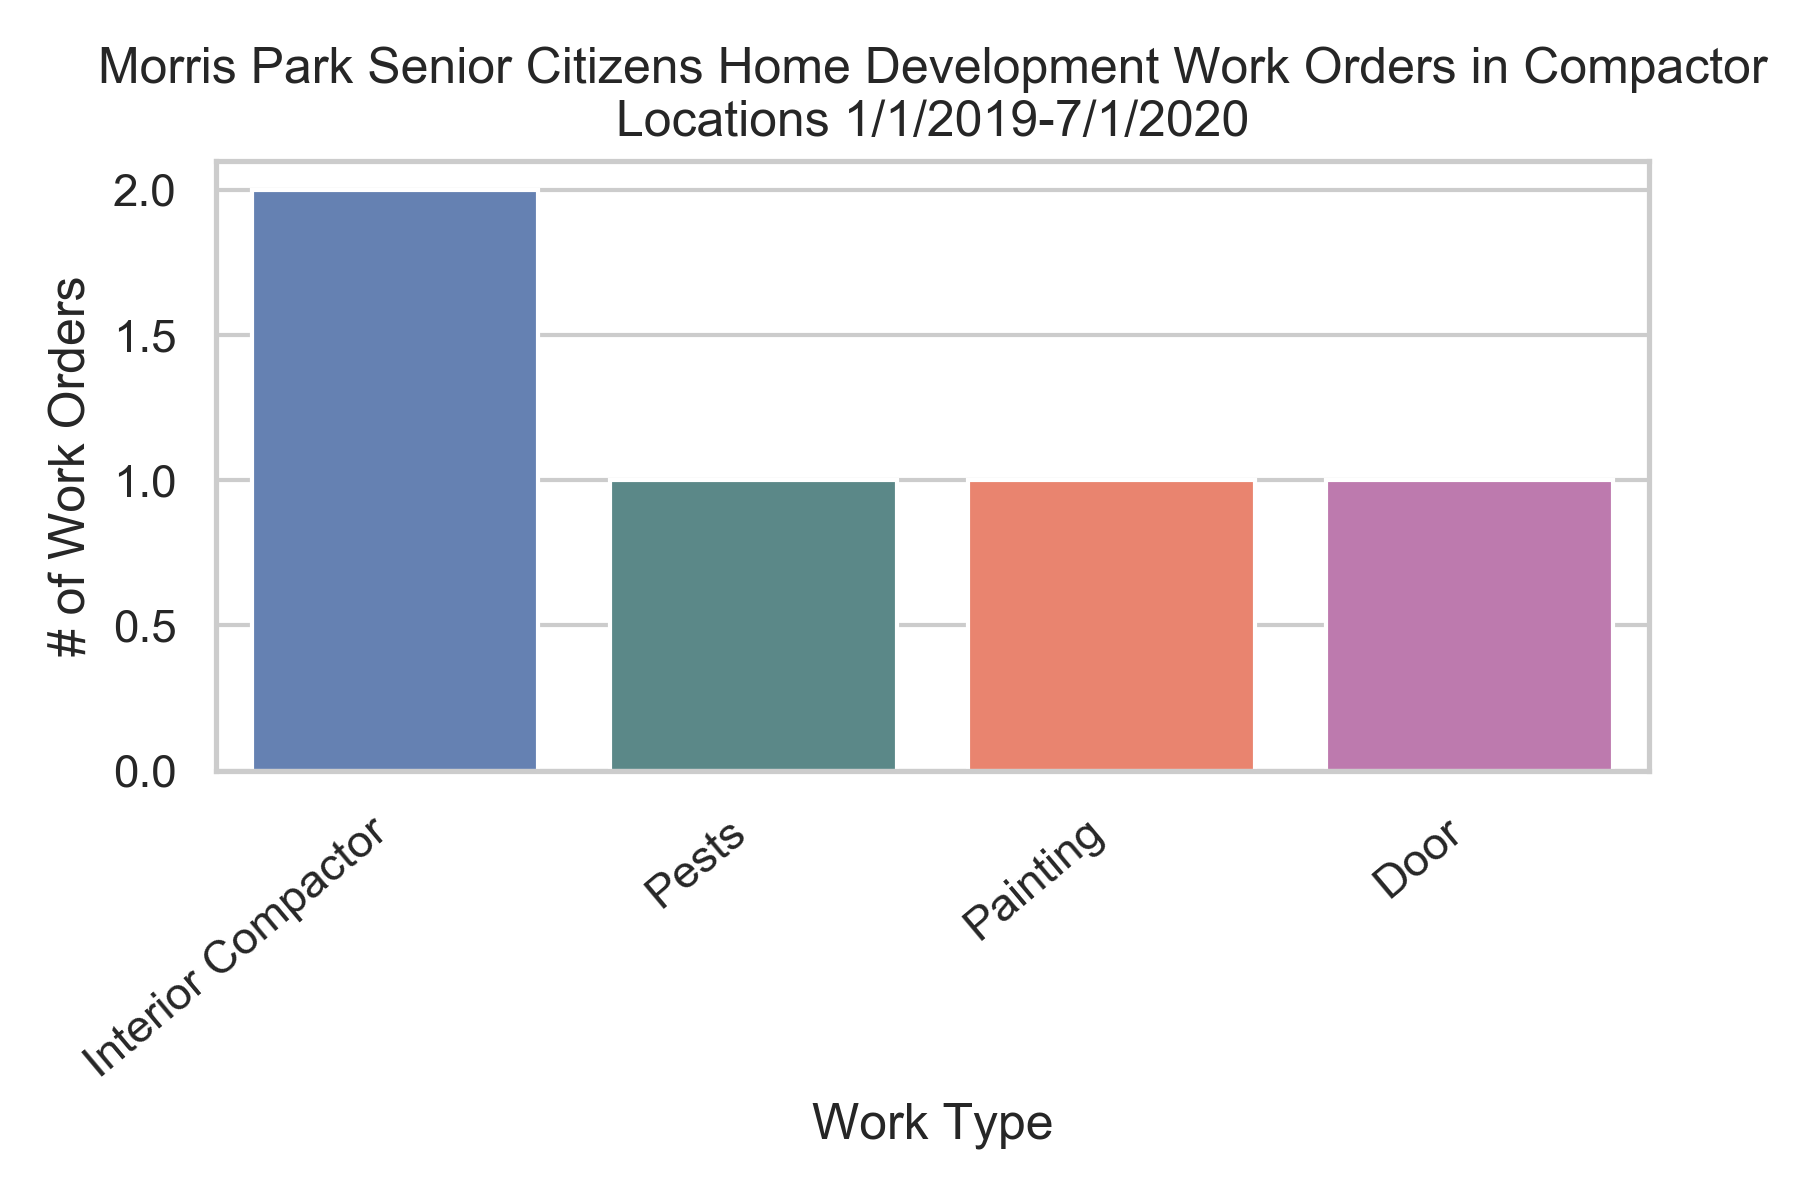
\includegraphics[width=0.45\textwidth]{\rootpath/WORK_ORDER_ANALYSIS/Development_BarCharts/png/277_MORRIS-PARK-SENIOR-CITIZENS-HOME_WorkOrder_Category_BarChart.png} & 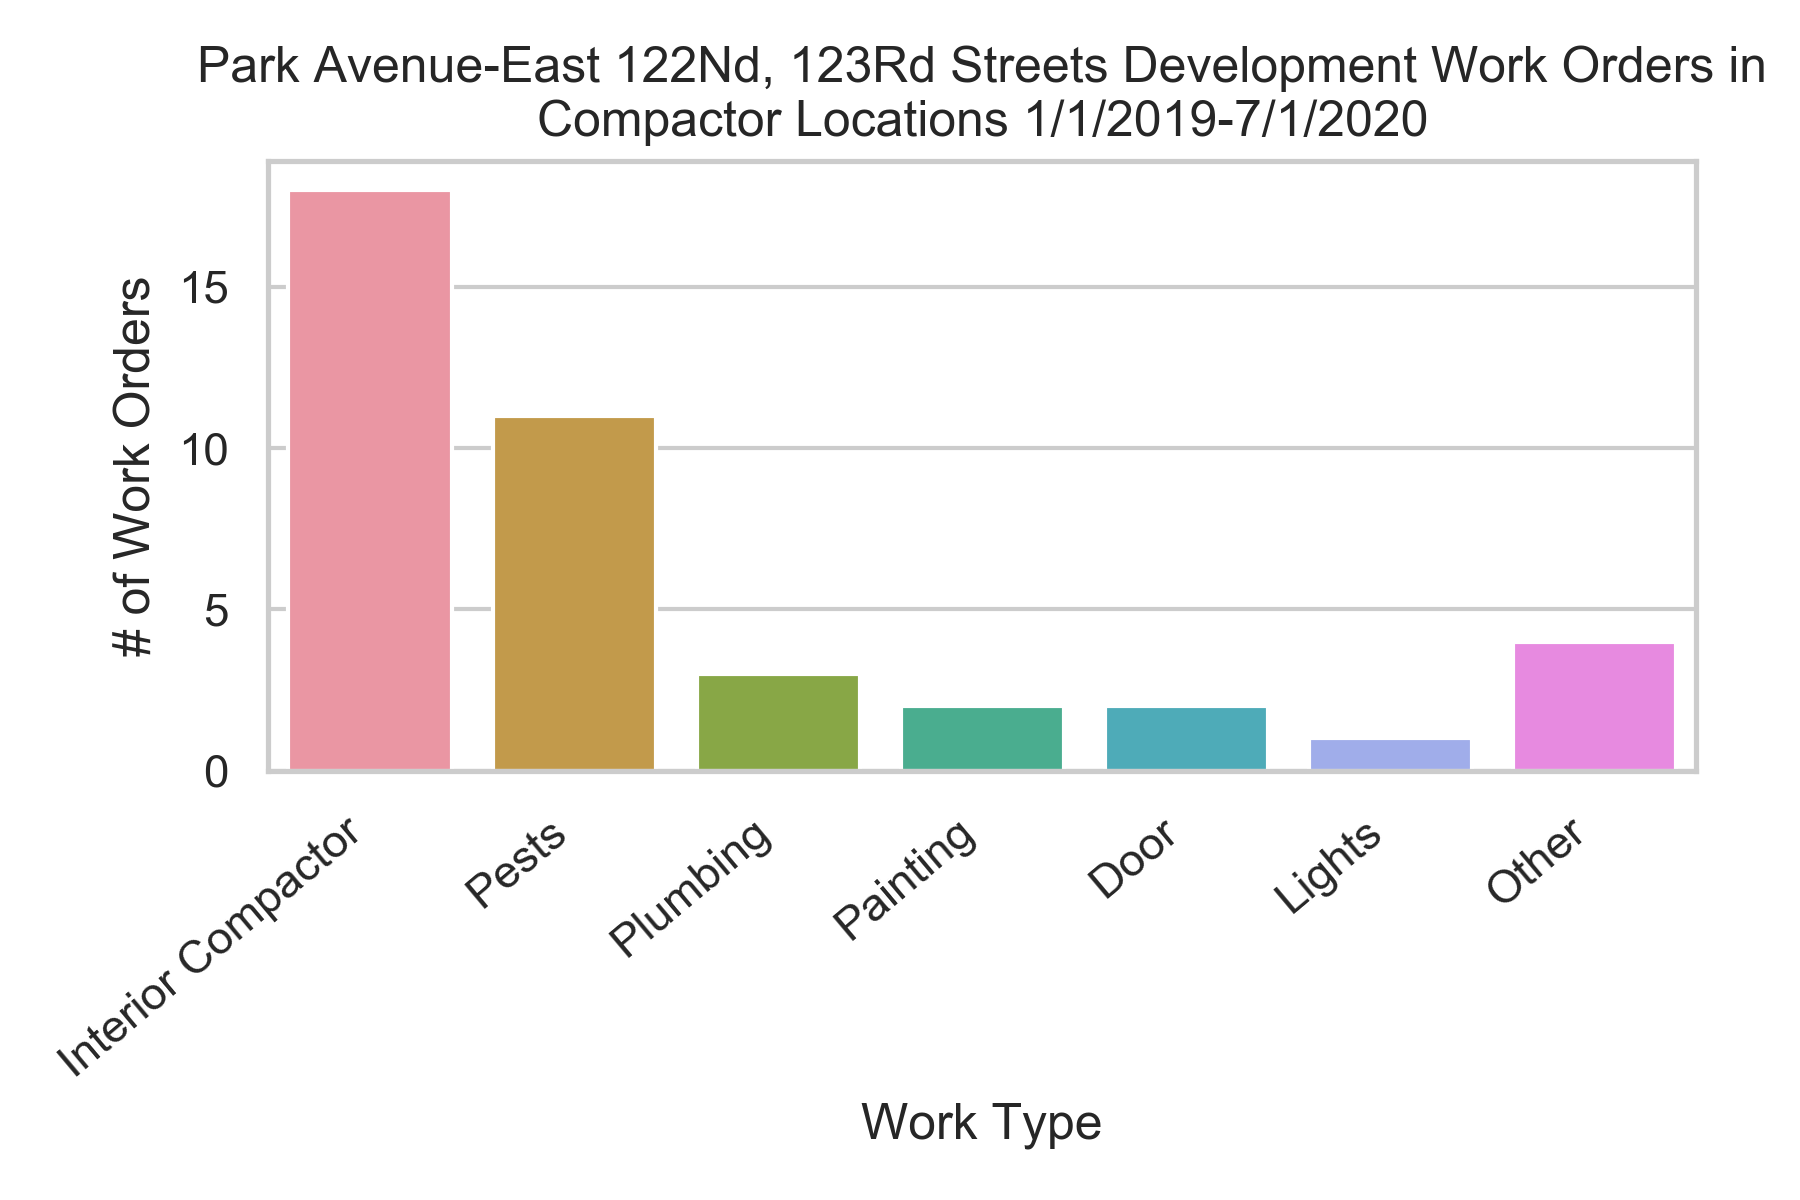
\includegraphics[width=0.45\textwidth]{\rootpath/WORK_ORDER_ANALYSIS/Development_BarCharts/png/204_PARK-AVENUE-EAST-122ND,-123RD-STREETS_WorkOrder_Category_BarChart.png} \\
                                        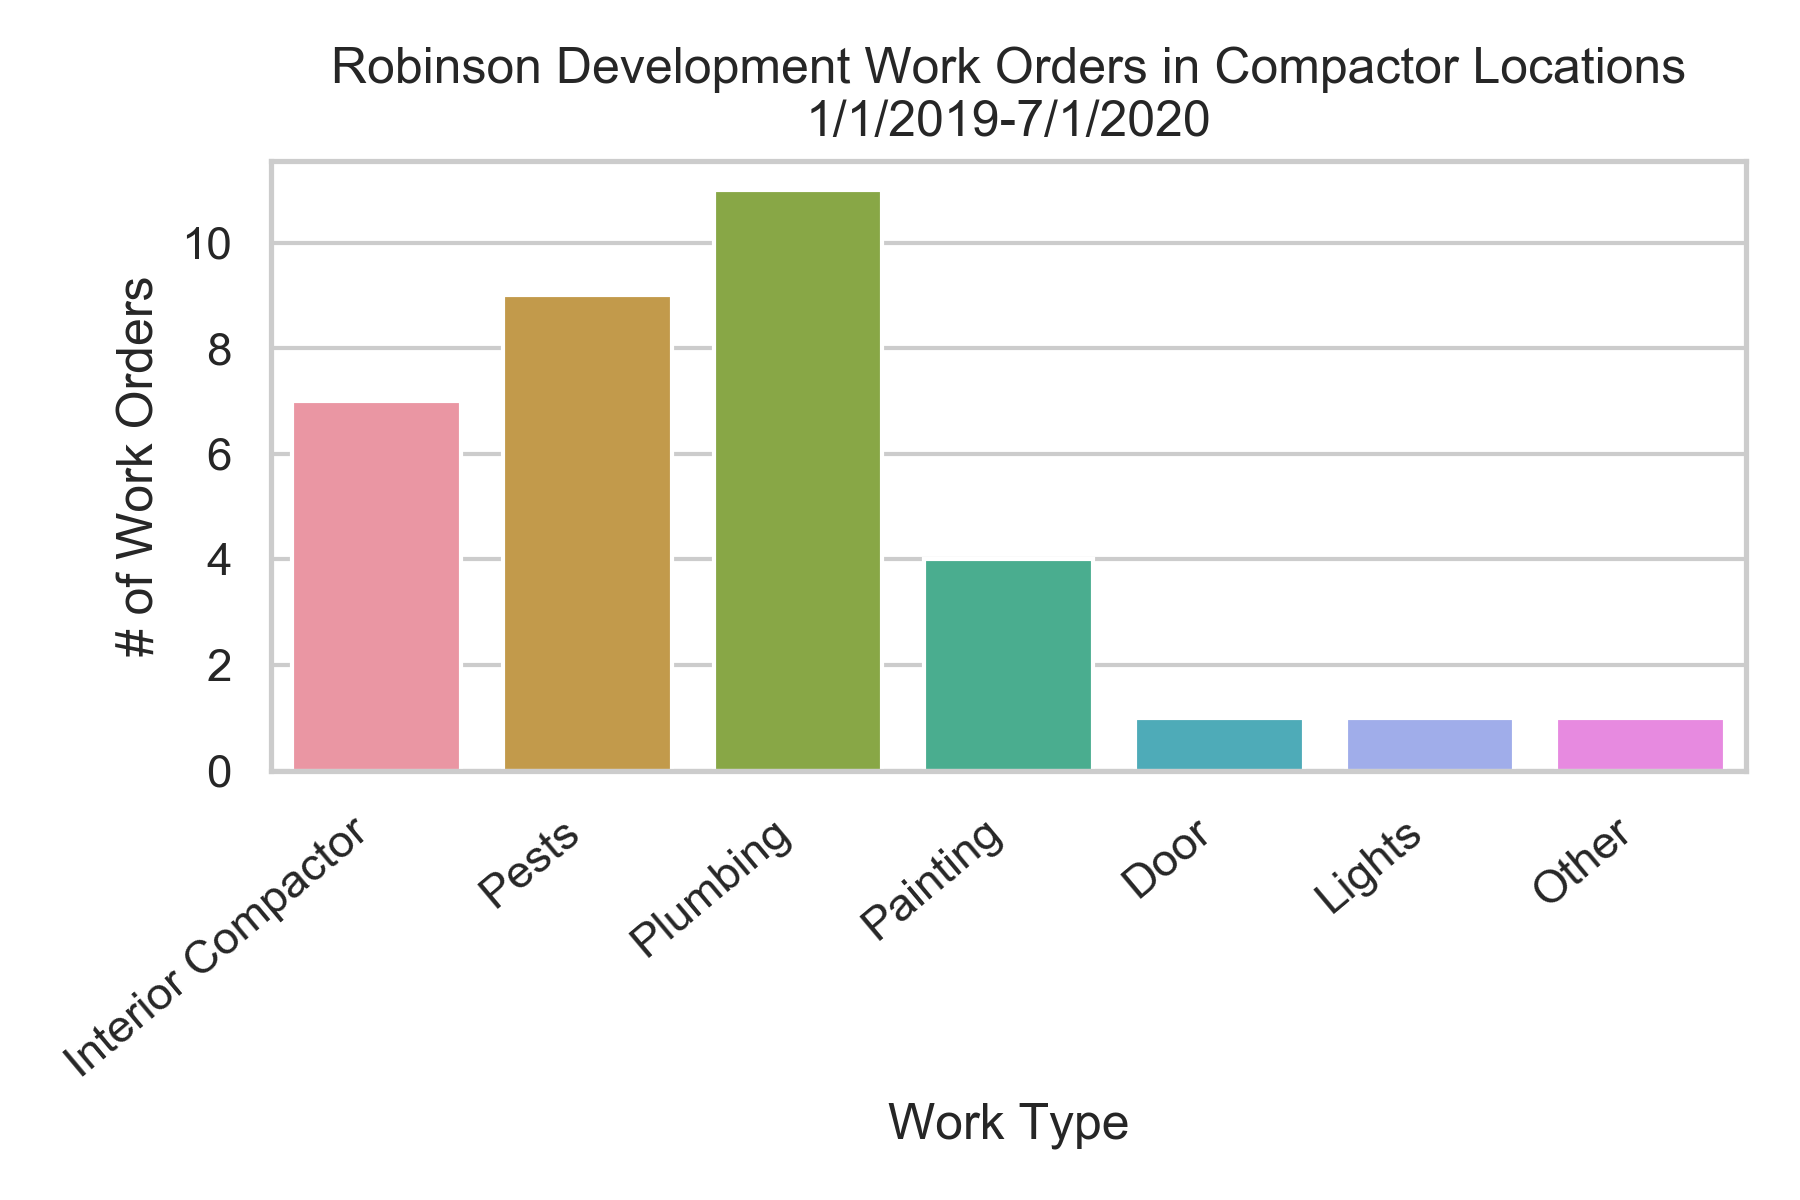
\includegraphics[width=0.45\textwidth]{\rootpath/WORK_ORDER_ANALYSIS/Development_BarCharts/png/241_ROBINSON_WorkOrder_Category_BarChart.png} & 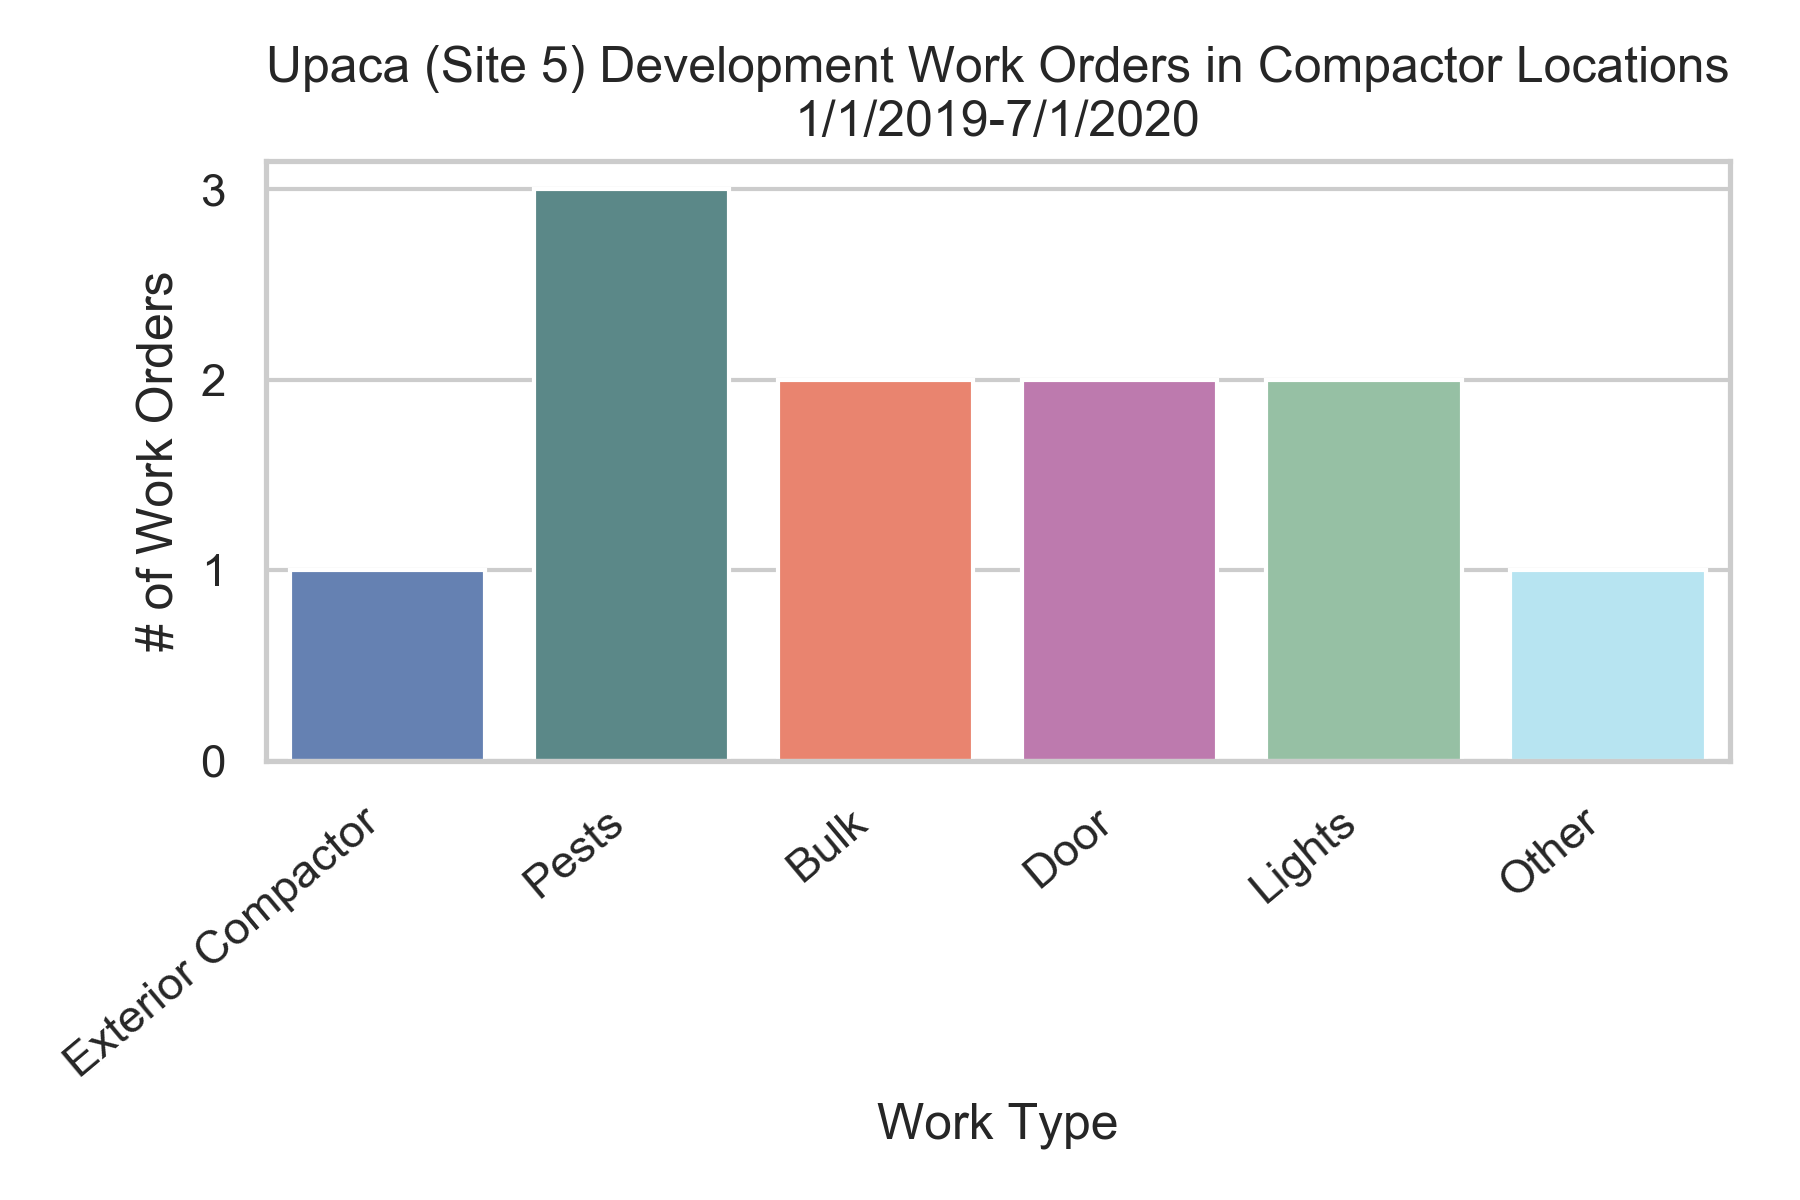
\includegraphics[width=0.45\textwidth]{\rootpath/WORK_ORDER_ANALYSIS/Development_BarCharts/png/343_UPACA-(SITE-5)_WorkOrder_Category_BarChart.png} \\
                                        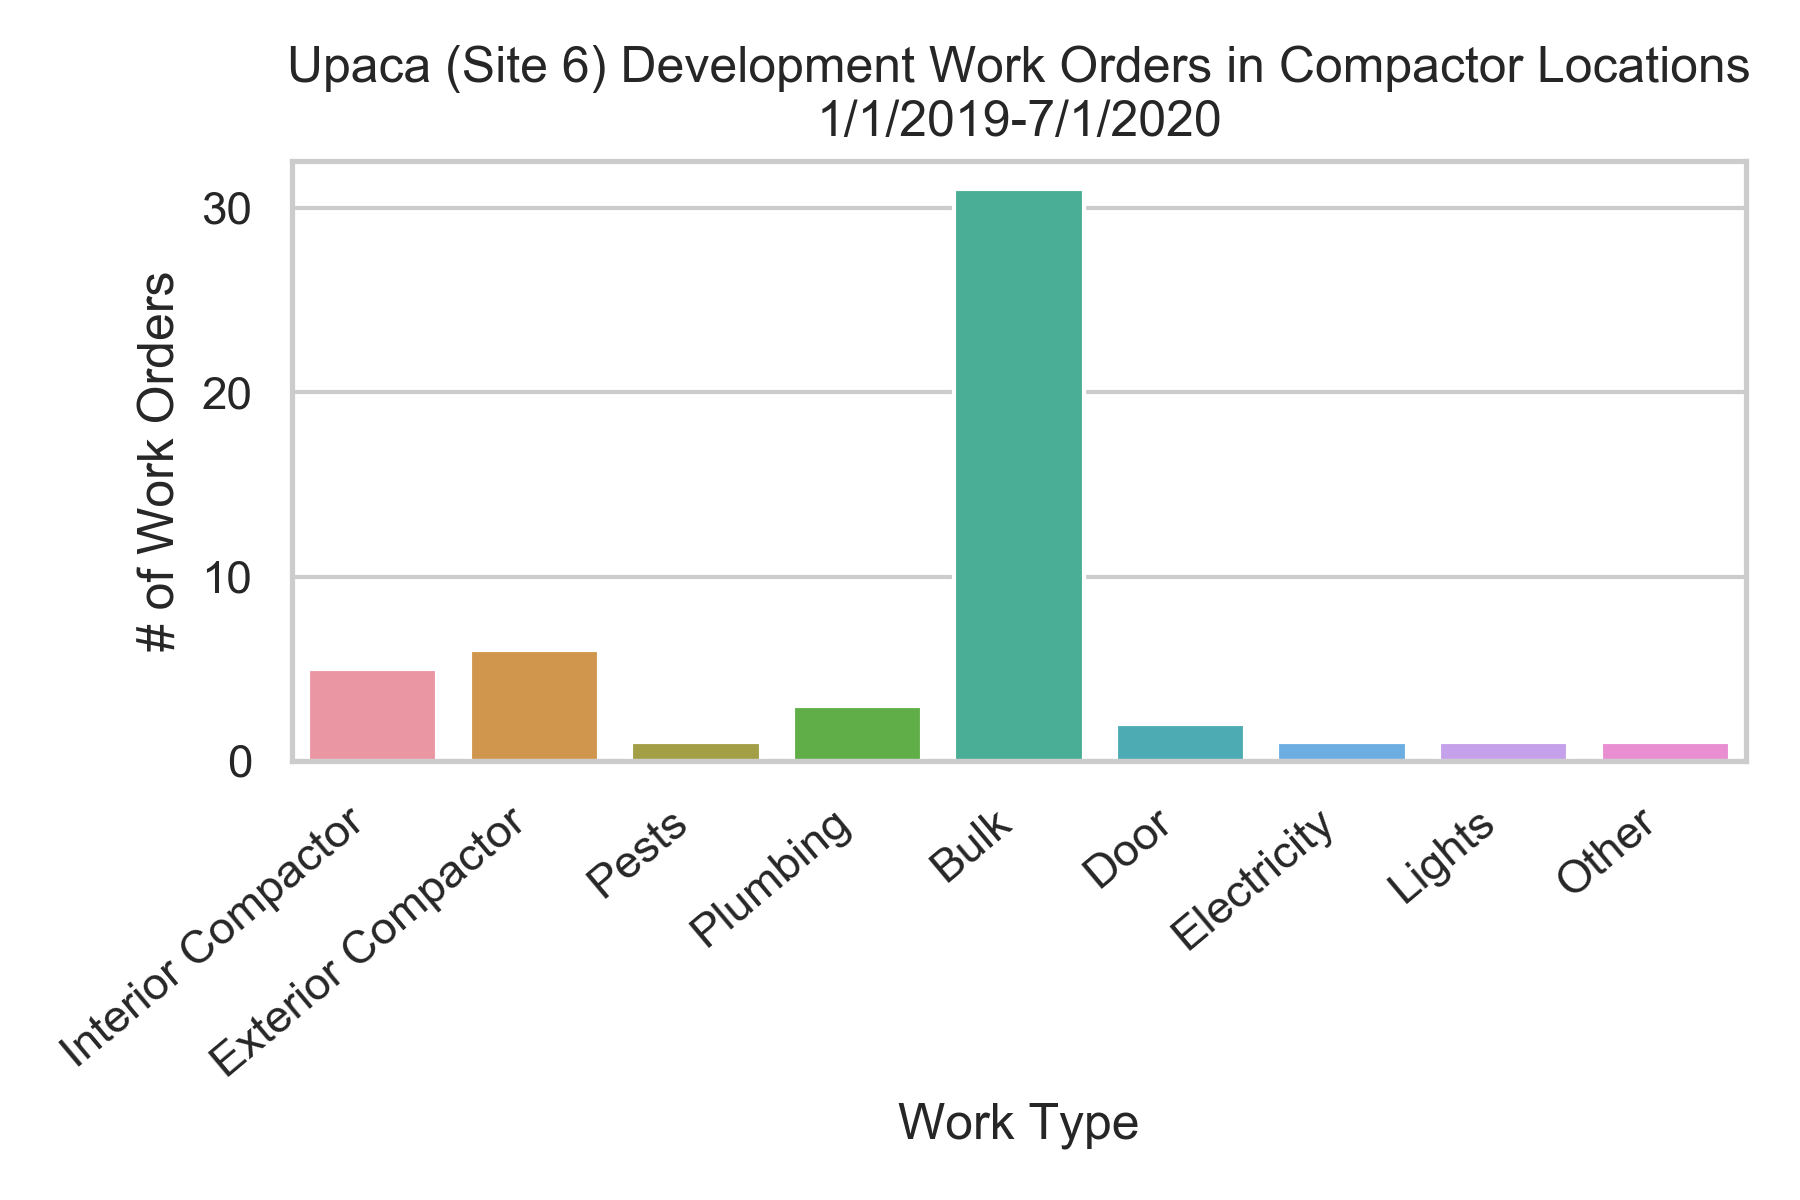
\includegraphics[width=0.45\textwidth]{\rootpath/WORK_ORDER_ANALYSIS/Development_BarCharts/png/355_UPACA-(SITE-6)_WorkOrder_Category_BarChart.png} &  \hspace{1cm} \\
                                        \end{supertabular}
\end{center}

                        \begin{center}
                        \tablehead{\hspace{1cm}\\}
                        \tabletail{\hspace{1cm}\\}
                        \begin{supertabular}{p{0.5\textwidth}p{0.5\textwidth}}
                        \multicolumn{2}{p{\textwidth}}{The following figures highlight repairs conducted in interior compactor locations at each major development, as well as within up to five buildings at each development.} \\
                        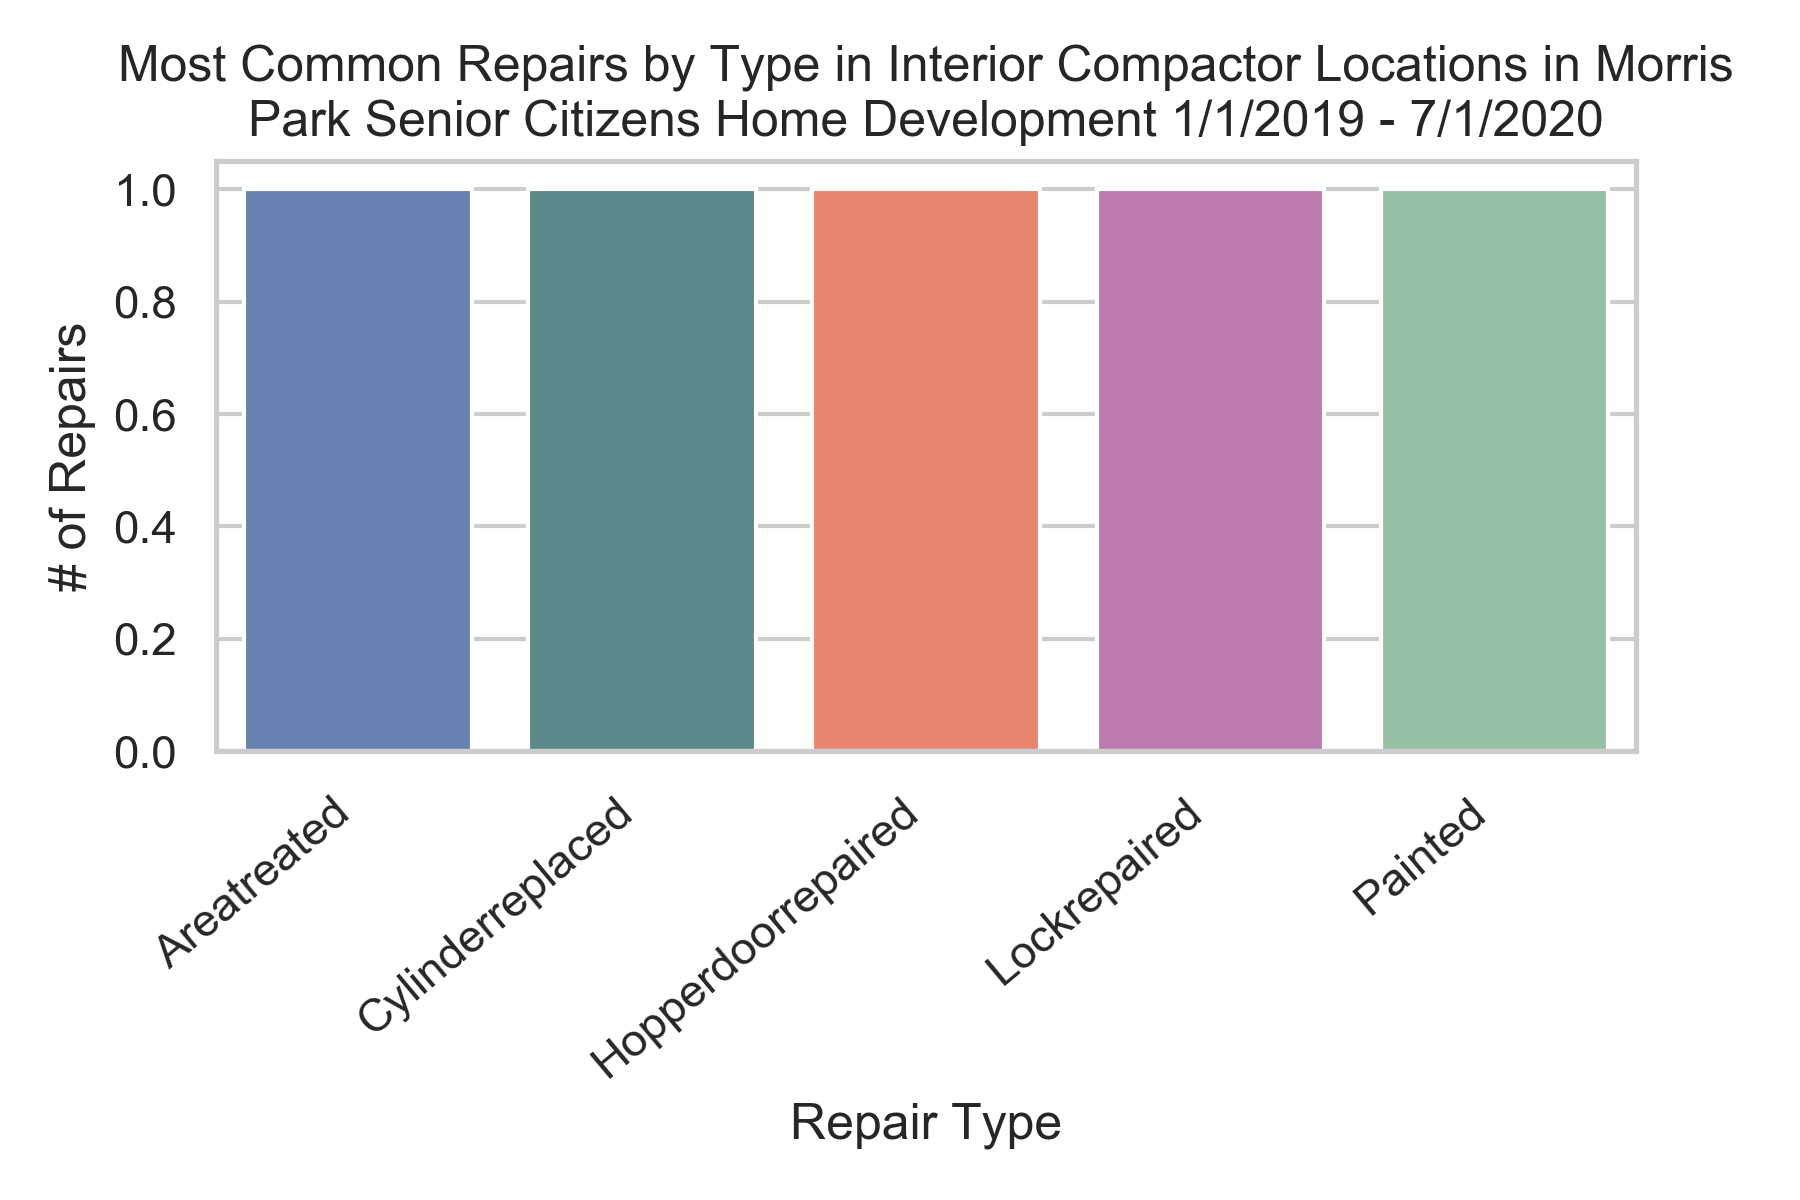
\includegraphics[width=0.45\textwidth]{\rootpath/WORK_ORDER_ANALYSIS/Dev_Interior_Comp_Repair_BarCharts/png/Jackie-Robinson_241_Morris-Park-Senior-Citizens-Home_277_Interior_Comp_Rep_BarChart.png} & 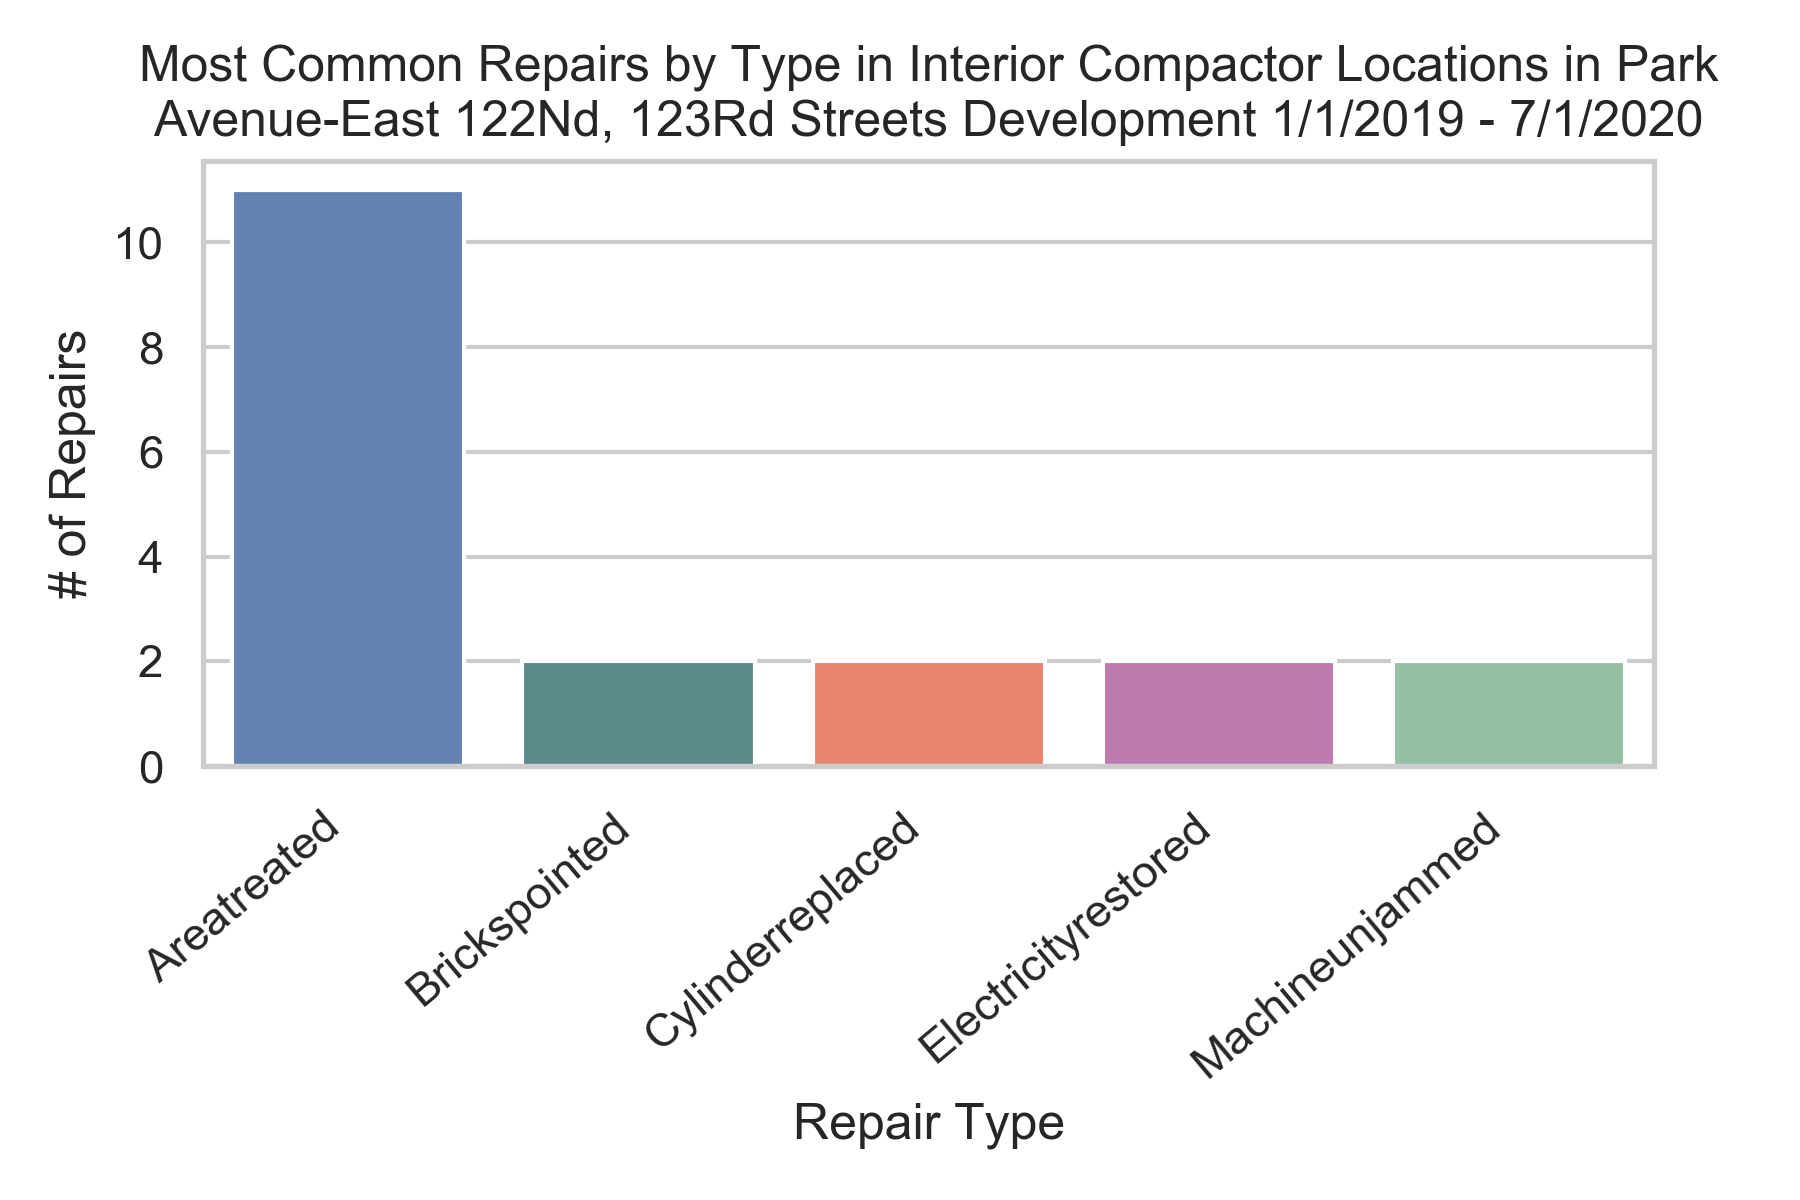
\includegraphics[width=0.45\textwidth]{\rootpath/WORK_ORDER_ANALYSIS/Dev_Interior_Comp_Repair_BarCharts/png/Jackie-Robinson_241_Park-Avenue-East-122Nd,-123Rd-Streets_204_Interior_Comp_Rep_BarChart.png} \\
                                        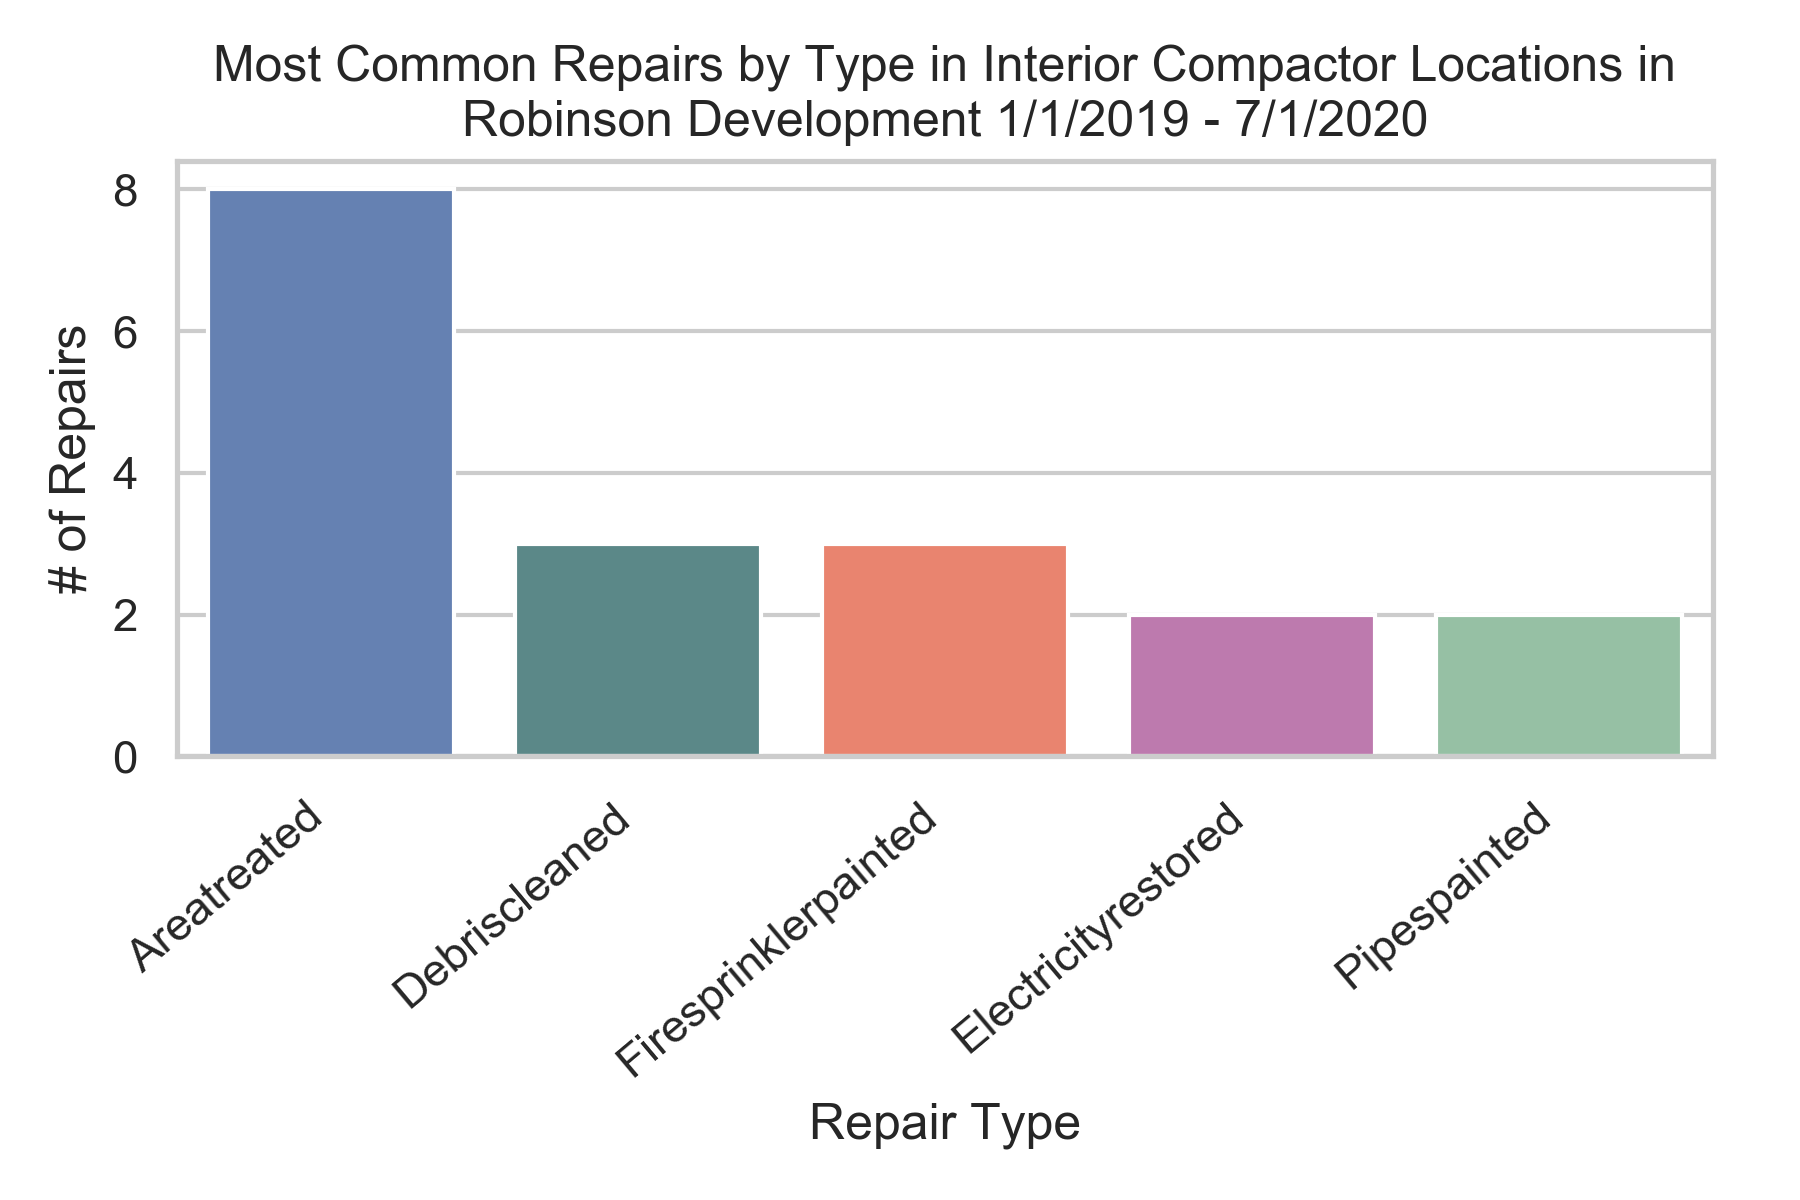
\includegraphics[width=0.45\textwidth]{\rootpath/WORK_ORDER_ANALYSIS/Dev_Interior_Comp_Repair_BarCharts/png/Jackie-Robinson_241_Robinson_241_Interior_Comp_Rep_BarChart.png} & 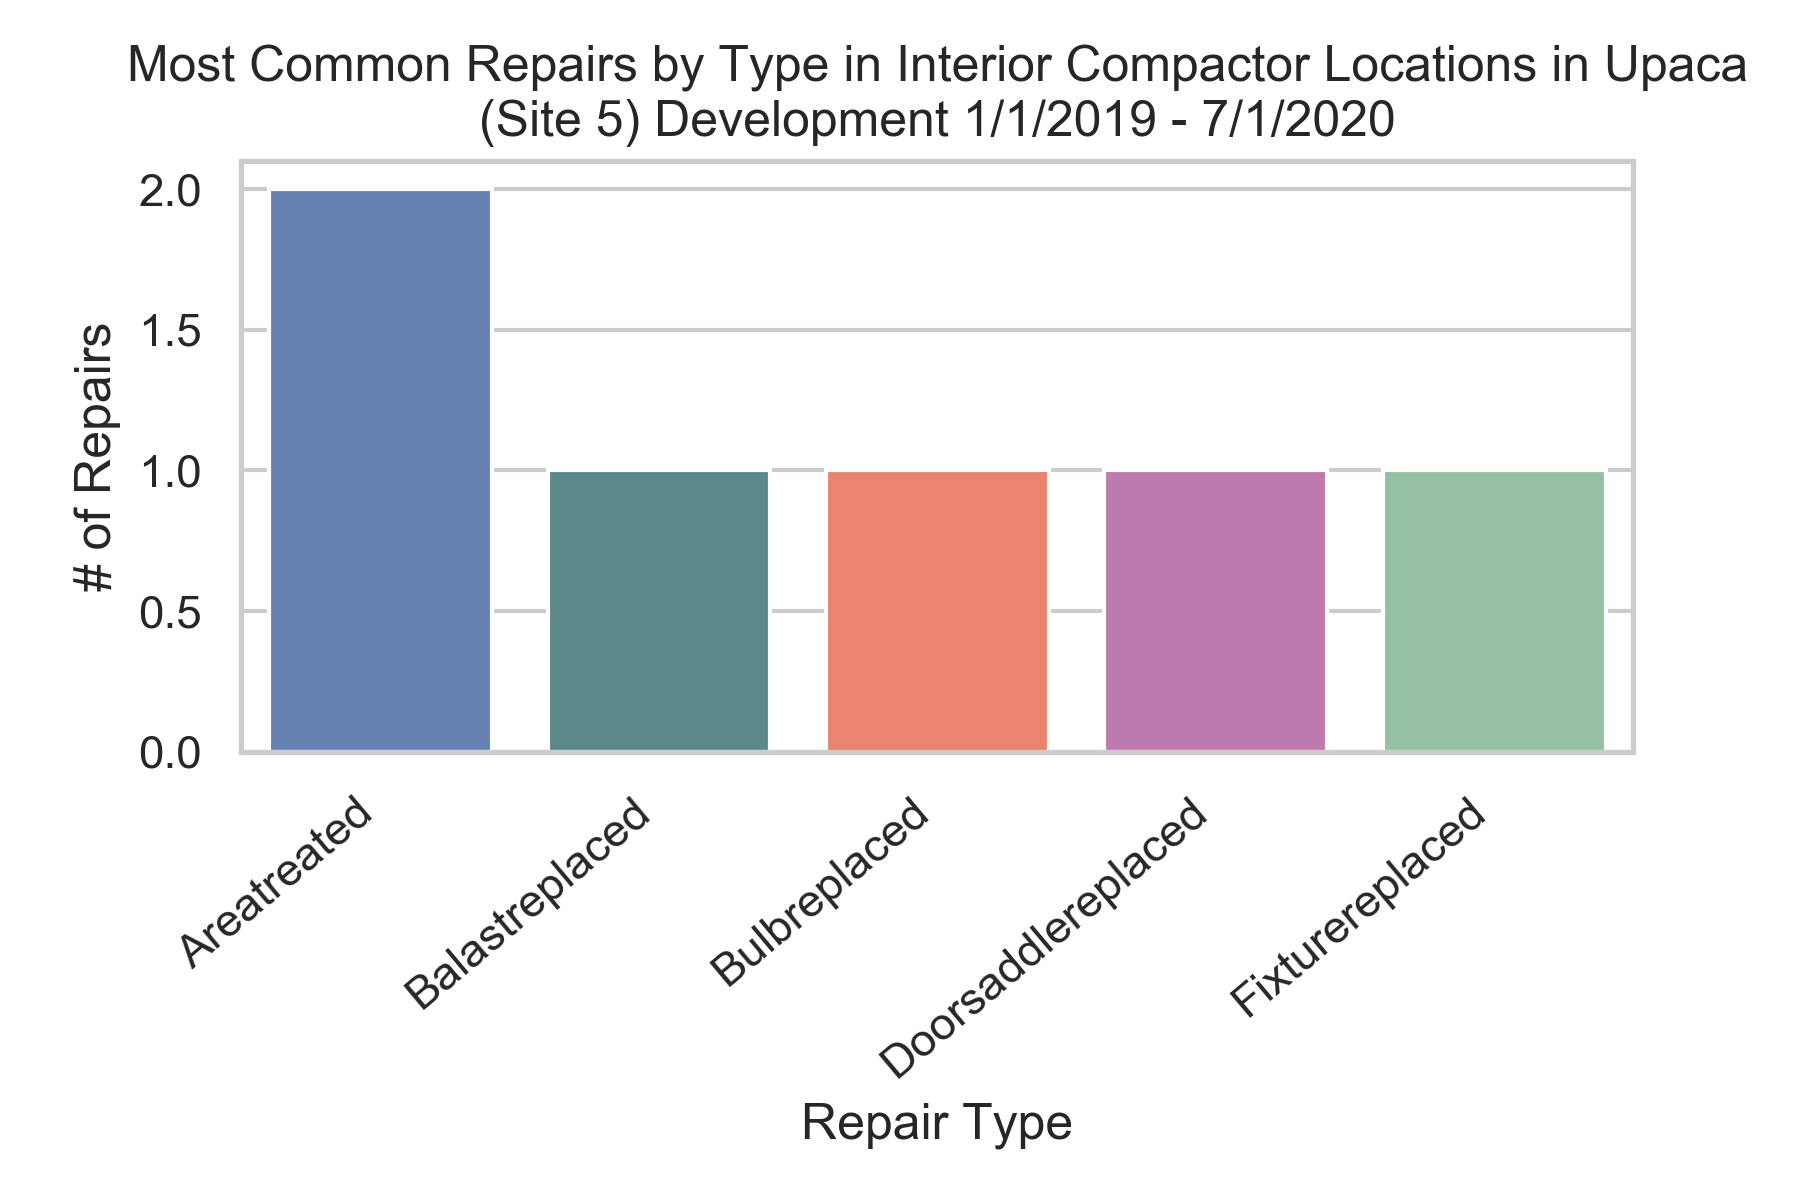
\includegraphics[width=0.45\textwidth]{\rootpath/WORK_ORDER_ANALYSIS/Dev_Interior_Comp_Repair_BarCharts/png/Jackie-Robinson_241_Upaca-(Site-5)_343_Interior_Comp_Rep_BarChart.png} \\
                                        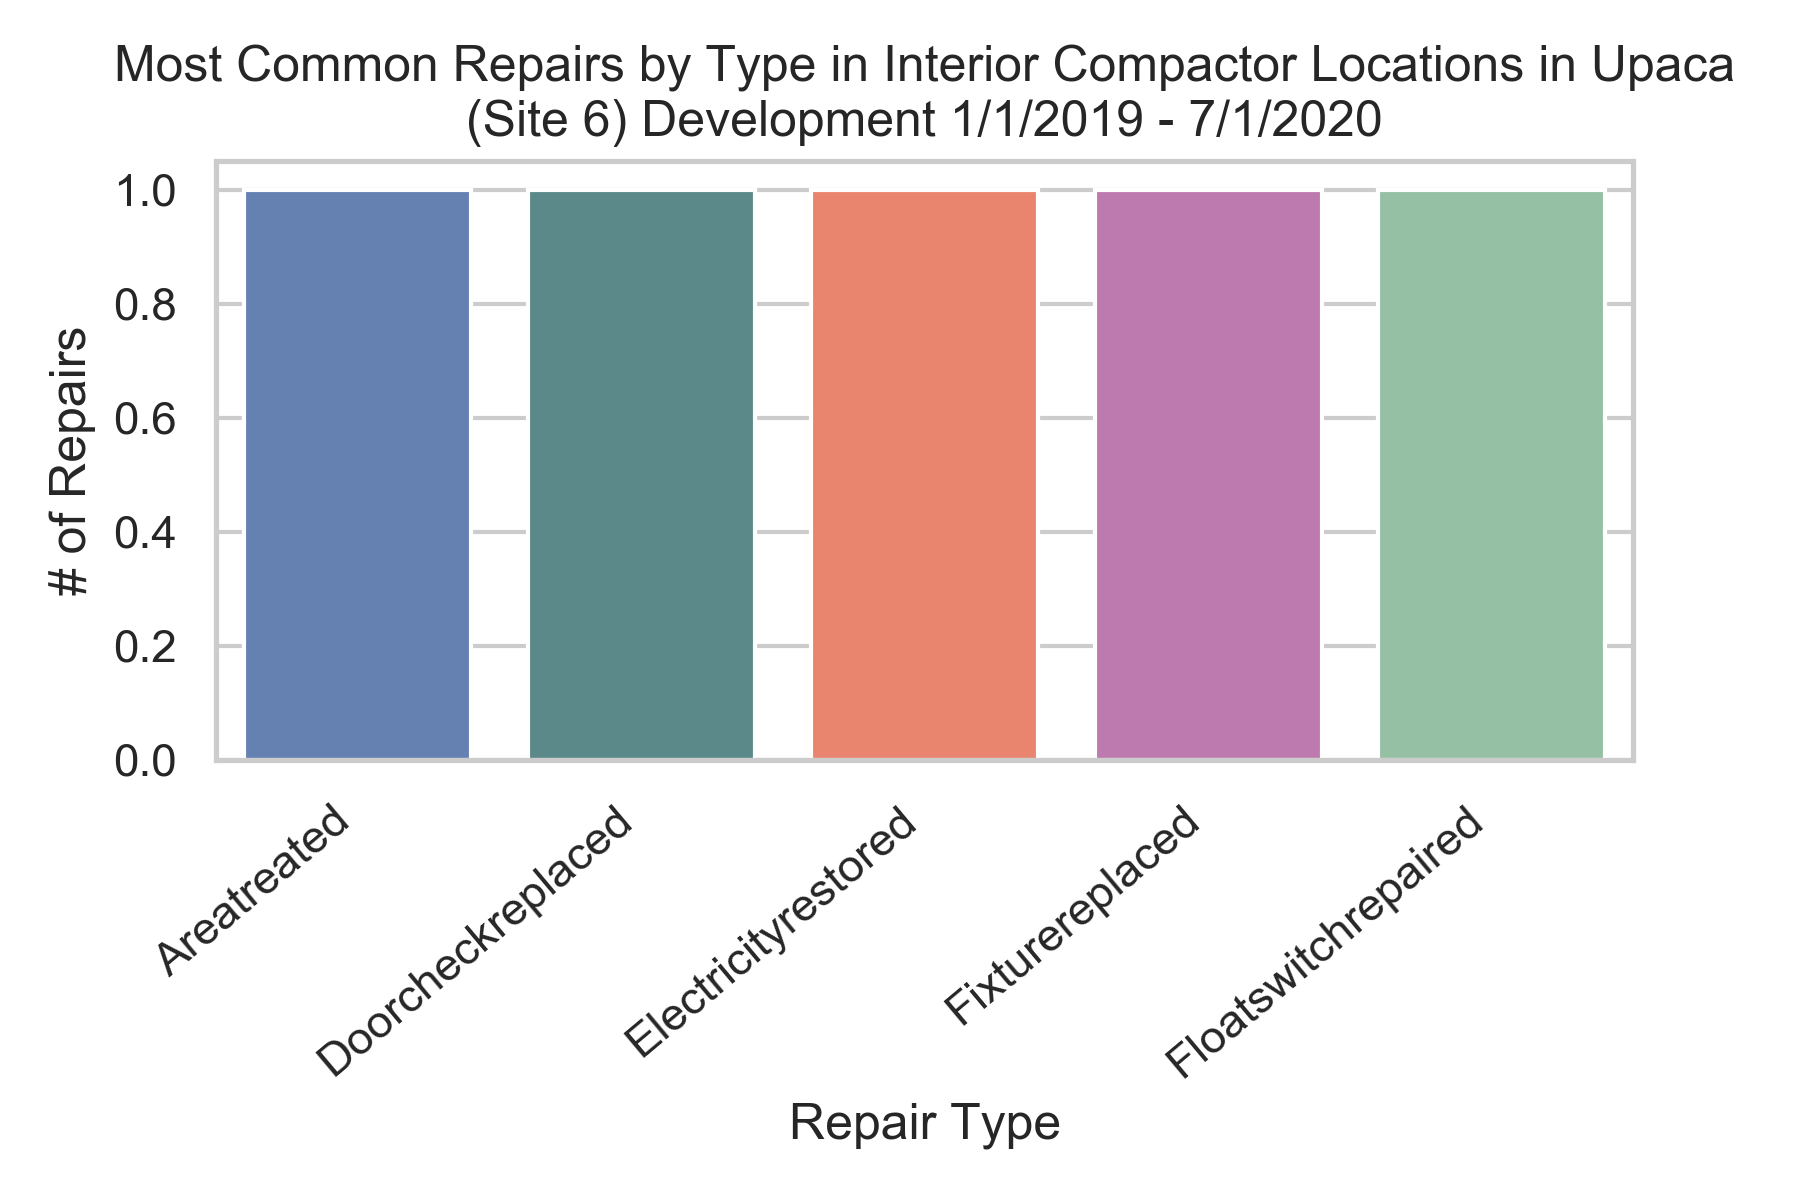
\includegraphics[width=0.45\textwidth]{\rootpath/WORK_ORDER_ANALYSIS/Dev_Interior_Comp_Repair_BarCharts/png/Jackie-Robinson_241_Upaca-(Site-6)_355_Interior_Comp_Rep_BarChart.png} &  \hspace{1cm} \\
                                        \multicolumn{2}{c}{\input{\rootpath/WORK_ORDER_ANALYSIS/Dev_Interior_Comp_Repair_Tables/\tds_repair_table}} \\
\end{supertabular}
\end{center}

                        \begin{center}
                        \tablehead{\hspace{1cm}\\}
                        \tabletail{\hspace{1cm}\\}
                        \begin{supertabular}{p{0.5\textwidth}p{0.5\textwidth}}
                        \multicolumn{2}{p{\textwidth}}{The following chart examines repairs made at exterior compactor locations.} \\
                        \multicolumn{2}{c}{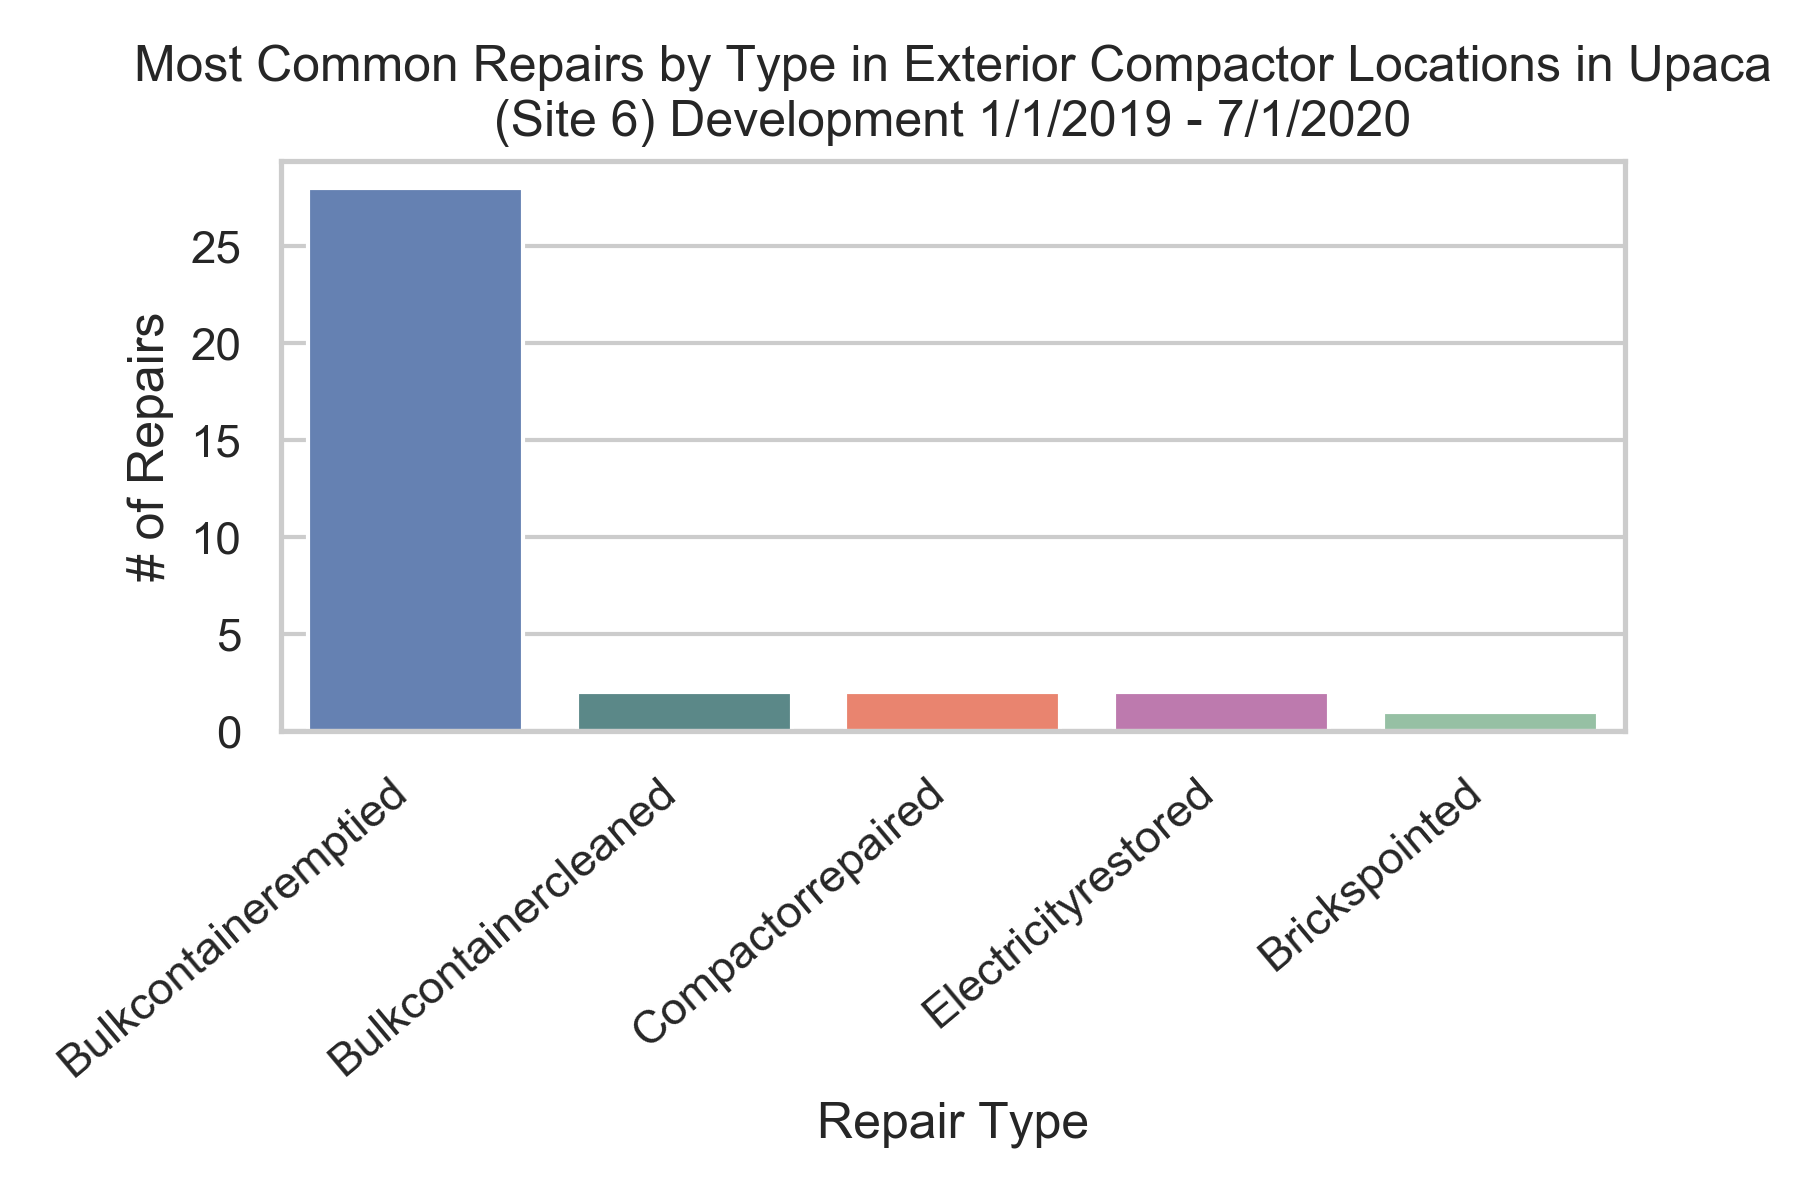
\includegraphics[width=0.6\textwidth]{\rootpath/WORK_ORDER_ANALYSIS/Dev_Exterior_Comp_Repair_BarCharts/png/Jackie-Robinson_241_Upaca-(Site-6)_355_Exterior_Comp_Rep_BarChart.png}} \\
                                    \end{supertabular}
                                    \end{center}
                                    